Esto modifica la distanncia de la onda en el eje $x$. Una fase negativa $(-)$ representa una distancia hacia la derecha y una positiva $(+)$ hacia la izquierda en el eje. Se representa usando la letra griega phi minúscula $(\phi)$.

\[\boxed{
  f(x)=\sin(x-\phi)
}\]

\begin{tikzpicture}
  \begin{axis}[
    xmin=0,xmax=2.2*pi,
    ymin=-1.2,ymax=1.2,
    axis lines=middle,
    % xtick={0},
    xtick={pi/2,pi,3*pi/2,2*pi},
    xticklabels={
      $\dfrac{\pi}{2}$,
      $\pi$,
      $\dfrac{3}{2}\pi$,
      $2\pi$
    },
    xticklabel style={anchor=south west},
    ytick={-1,1},yticklabels={$-1$,$1$}
    ]

    \addplot[color=red,samples=100,domain=0:2*pi,thick]{sin(deg(x))};

    \addplot[color=green,samples=100,domain=0:2*pi,thick]{sin(deg(x - 90))};

    \addplot[color=blue,samples=100,domain=0:2*pi,thick]{sin(deg(x - 180))};

    % \addplot[color=yellow,samples=100,domain=0:2*pi,thick]{sin(deg(x - 270))};

    % \legend{$\sin(x - \frac{\pi}{2})$, $\sin(x - \pi))$, $\sin(x - \frac{3}{2}\pi))$}
  \end{axis}
\end{tikzpicture}

Al cambiar la distancia de la onda se puede cambiar su patrón. La función $\sin(x)$ puede resultar en el patrón de una función $\cos(x)$ si se aplica la fase correcta. También puede ocurrir la contrario, convertir una función $\cos(x)$ en una función $\sin(x)$.

\begin{tikzpicture}
  \begin{axis}[
    xmin=0,xmax=2.2*pi,
    ymin=-1.2,ymax=1.2,
    axis lines=middle,
    ytick={0},
    xtick={pi/2,pi,3*pi/2,2*pi},
    xticklabels={
      $\dfrac{\pi}{2}$,
      $\pi$,
      $\dfrac{3}{2}\pi$,
      $2\pi$
    },
    xticklabel style={anchor=south west}
    ]

    \addplot[color=red,samples=100,domain=0:2*pi,thick]{cos(deg(x))};

    \addplot[color=green,samples=100,domain=0:2*pi,thick]{sin(deg(x))};

    \legend{$\cos(x)$,$\cos(x - \frac{\pi}{2})$}
  \end{axis}
\end{tikzpicture}

Se observa que al aplicar una fase de $\dfrac{\pi}{2}$ hacia la derecha en la función $\cos(x)$ se obtiene una función $\sin(x)$.

\begin{listequbox}
  {\sin(x)=\cos\left(x - \dfrac{\pi}{2}\right)}{equcosphasesin}{Identidad de $\cos(x - \frac{\pi}{2})$ y $\sin(x)$}
\end{listequbox}

Una relación parecida ocurre con el $\sin(x)$ al cambiar de fase en $\dfrac{\pi}{2}$ hacia la izquierda, se obtiene $\cos(x)$.

\begin{tikzpicture}
  \begin{axis}[
    xmin=0,xmax=2.2*pi,
    ymin=-1.2,ymax=1.2,
    axis lines=middle,
    ytick={0},
    xtick={pi/2,pi,3*pi/2,2*pi},
    xticklabels={
      $\dfrac{\pi}{2}$,
      $\pi$,
      $\dfrac{3}{2}\pi$,
      $2\pi$
    },
    xticklabel style={anchor=south west}
    ]

    \addplot[color=blue,samples=100,domain=0:2*pi,thick]{sin(deg(x))};

    \addplot[color=orange,samples=100,domain=0:2*pi,thick]{cos(deg(x))};

    \legend{$\sin(x)$,$\sin(x + \frac{\pi}{2})$}
  \end{axis}
\end{tikzpicture}

\begin{listequbox}
  {\cos(x)=\sin\left(x + \dfrac{\pi}{2}\right)}{equsinphasecos}{Identidad de $\sin(x + \frac{\pi}{2})$ y $\cos(x)$}
\end{listequbox}
